
%We consider a \emph{listener} who, as the speaker's utterance unfolds, engages in incremental prediction.
%%Informally, we expect that both speaker and listener will be affected by memory demands:
%%rom the speaker's perspective, producing well-formed sentences will require information about what she has uttered so far.
%For the listener, predicting the next word well requires maintaining information about the past.
%For the listener, the quality of prediction is measured by the average \emph{surprisal} experienced.
%For a fixed language, we can ask how much information about the past (1) the speaker has to maintain to produce well-formed utterances, and (2) the listener has to maintain to incur a minimal amount of surprisal.
%Utilizing the tools of information theory, we quantify memory in \emph{bits}, obtaining bounds that hold across different models of memory architecture and ways of quantifying memory load.
%
%
%TODO say at some point that we're studying sentence-internal memory



\begin{figure}
\centering
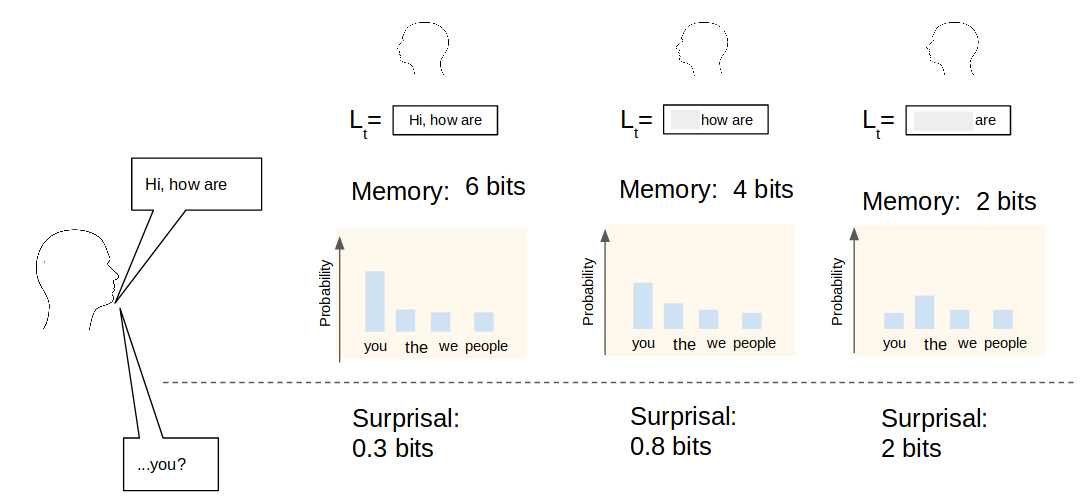
\includegraphics[width=0.9\textwidth]{figures-gdrive/communication.png}
	\caption{Memory and language comprehension. (1) A speaker produces a sequence of words. (2) A listener maintains a representation of the words received so far. The listener can represent these at higher (left) or lower (right) levels of precision. (3) Throughout communication, the listener generates probabilistic expectations about the next word. Higher precision of memory representations leads to more precise predictions. (4) When receiving the next word, the listener incurs surprisal depending on the predictions. Higher levels of fidelity in memory lead to lower surprisal on average. \jd{what do the numbers (1) (2) etc refer to? also: image is blurry, at least on my screen}\note{make reference to $L_t$ inside the caption. you and the surprisals visually better aligned. maybe can color-code? } \mhahn{problem suggests that memory has to be contiguous substrings}}
	\label{fig:communication}
\end{figure}

We begin developing our model by considering the process of language comprehension illustrated in Figure~\ref{fig:communication}, where the listener Alice is processing a stream of words uttered by an interlocutor Bob (Figure~\ref{fig:communication}).


Experimental research has established that (1) listeners maintain information about the words received so far, (2) listeners forms probabilistic expectations about the upcoming words, and (3) words are easy to process to the extent that they are predictable in context \rljf{Good source for other cites here would be to dig around in Luke \& Christianson's review of predictability effects}. Furthermore, the exact mathematical form of the relationship between predictability and processing difficulty (as measured e.g. in reading times) seems to be given by the \key{information content} of a word in context \cite{hale2001probabilistic,levy2008expectation,smith2013effect}.


Surprisal theory \citep{hale-probabilistic-2001, levy-expectation-based-2008} posits that the processing effort on a word $w_t$ in context $w_1\dots w_{t-1}$ is proportional to the \key{surprisal} of the word in context:
\begin{equation}
S = -\log \operatorname{P}(w_t|w_1\dots w_{t-1})\label{eq:surp}.
\end{equation}
Experimental work has confirmed that surprisal is a reliable and linear predictor of processing effort as reflected in reading times \citep{smith-effect-2013}.

The average processing difficulty associated with a language then comes out to its entropy rate:
\begin{equation}
	S = \operatorname{H}(w_t|w_1\dots w_{t-1}).
\end{equation}



However, surprisal theory as presented above cannot in principle account for effects of memory limitations on online processing, because Equation~\ref{eq:surp} represents surprisal as experienced by an idealized listener who accurately remembers the entire history of previous words $w_{1...t-1}$.
More realistically, human listeners deploy memory resources that maintain imperfect representations of the preceding context \citep{lewis-activation-based-2005, futrell-noisy-context-2017}.
If $m_{t-1}$ is a listener's memory state after hearing $w_1\dots w_{t-1}$, then the true surprisal experienced by the listener will be:
\begin{equation}
  \label{eq:lossy-surp}
  S_M := -\log_2 \operatorname{P}(x_t|m_{t-1}),
\end{equation}
which must be larger than Eq.~\ref{eq:surp} on average (see below for proof).
This modified surprisal $S_M$ in Eq.~\ref{eq:lossy-surp} can account for well-known memory effects on online processing such as dependency locality effects and structural forgetting \citep{futrell-noisy-context-2017,futrell2019information}.
The limitations of memory have well-documented empirical effects on language processing, causing difficulty above and beyond the difficulty associated with raw information content \cite{gibson1998linguistic,gibson1999memory,gibson2000dependency,vasishth2005activationbased,levy2013memory}.

The average processing difficulty associated with a language then comes out to a \key{cross entropy}:
\begin{equation}
	S = \operatorname{H}(w_t|m_{t-1}).
\end{equation}


These considerations imply a \emph{tradeoff between memory and surprisal}:
A listener maintaining higher-precision memory representations $m_{t-1}$ will, on average, incur lower surprisal, at the cost of higher memory load.
The idea of the memory-surprisal tradeoff is visualized in Fig.~\ref{fig:tradeoff}: for each desired level of average surprisal, there is a minimum number of bits of information which must be stored about context.
The shape of the trade-off is determined by the language, and in particular its word order:
some languages enable more efficient trade-offs than others by forcing a listener to store more bits in memory to achieve the same level of average surprisal.


Here we propose to model human language comprehension by treating the listener's memory $m_{i-1}$ as a lossily compressed representation of the context $x_{1...i-1}$, and the processing effort associated with each word using Eq.~\ref{eq:lossy-surp}.
Suppose that the listener's memory has a fixed information-carrying capacity $k$, then this listener has to compress the context into a memory representation $m_{i-1}$ with at most $k$ bits: $H[m_{i-1}] \leq k$.
Information theory implies that the processing cost $S_M$ trades off with the memory capacity $k$:
Processing cost will be lower for a listener who represents past input at higher levels of precision.




We prove a theorem describing how the shape of this tradeoff relates to language structure. %relating memory to the experienced comprehension difficulty $S$.
%Informally, the theorem says that languages support more efficient tradeoffs between short-term memory and comprehension difficulty when words are strongly predictive of their neighboring words.
This theorem captures formally that languages support more efficient tradeoffs between short-term memory and comprehension difficulty when words are strongly predictive of their neighboring words.


We derive the precise form of the memory-surprisal tradeoff in Theorem 1.
Let $\operatorname{I}_t$ be the conditional mutual information between words that are $t$ steps apart, conditioned on the intervening words: 
\begin{equation}
	\operatorname{I}_t := \operatorname{I}[w_t, w_0 | w_1, \dots, w_{t-1}] = \operatorname{H}[w_t|w_1, \dots, w_{t-1}] - \operatorname{H}[w_t|w_0, \dots, w_{t-1}] 
\end{equation}

This quantity measures how much predictive information the word $t$ steps in the past contains about the current word, above and beyond the information contained in the intervening words.

This is equal to the reduction in uncertainty about the $t$-th observation when knowing the $0$-th observation, in addition to the block of intervening observations.
That is, we measure the amount of statistical dependency of observations that are $t$ steps apart, controlling for any information that is redundant with intervening observations.
This quantifies how much information needs to be carried across $t$ timesteps without any possibility for `guessing' it from intervening observations.

This quantity, visualized in Figure~\ref{fig:theorem} (a), measures how much predictive information is provided by the next word $w_t$ by the word $t$ steps in the past.
It is a statistical property of the language, and can be estimated from large-scale text data.


Our theoretical results describe how the tradeoff between memory and comprehension difficulty relates to $I_t$ (Figure~\ref{fig:theorem} (b)):
Consider a listener who invests $B$ bits of memory into representing past input.
We then consider the smallest $T$ such that the area under the curve of $t I_t$, to the left of $T$, has size $B$.
Such a listener will experience average surprisal at least $H[w_t| w_{<t}] + \sum_{t=T+1}^\infty I_t$. %\note{maybe result first, and then say what $T$ is}
By tracing out all values $T >0$, one can obtain a bound on the tradeoff curve for any possible listener.

This is formalized in the following theorem:

\begin{thm}\label{prop:suboptimal}
Let $T$ be a positive integer, and consider a listener using at most $\sum_{t=1}^T t \operatorname{I}_t$ bits of memory on average.
Then this listener will incur average surprisal at least
$\operatorname{H}[w_t|w_{<t}] + \sum_{t > T} \operatorname{I}_t$.
\end{thm}


\begin{enumerate}
\item Ingredient 1: Language as a Stationary Stochastic Process:
We represent language as a stochastic process of words $\dots w_{-2} w_{-1} w_0 w_{1} w_{2} \dots$, extending indefinitely both into the past and into the future.
The symbols $w_i$ belong to a common set, representing the words of the language.\footnote{Could also be phonemes, sentences, ..., any other kind of unit.}

%We model the sequence as a probabilistic sequence; that is, given a context $w_{<t}$, the next word is distributed according to a distribution $p(w_t|w_{<t})$.

The assumption of infinite length is for mathematical convenience and does not affect the substance of our results:
As we restrict our attention to the processing of individual sentences, which have finite length, we will actually not make use of long-range and infinite contexts.

We make the assumption that this process is \emph{stationary}.
Formally, this means that the conditional distribution $P(w_t|w_{<t})$ does not depend on $t$, it only depends on the actual sequence $w_{<t}$.
Informally, this says that the process has no `internal clock', and that the statistical rules of the language do not change at the timescale we are interested in.
In reality, the statistical rules of language do change: They change as language changes over generations, and they also change between different situations -- e.g., depending on the interlocutor at a given point in time.
Given that we are interested in memory needs in the processing of \emph{individual sentences}, at a timescale of seconds or minutes, stationarity seems to be a reasonable assumption to make.

\item Ingredient 2: Flow of Information: We now analyze memory from the perspective of the listener, who needs to maintain information about the past to predict the future.
As the speaker's utterance unfolds, the listener maintains a memory state $m_t$.

There are no assumptions about the memory architecture and the nature of its computations.
We only make a basic assumption about the flow of information (Figure~\ref{fig:listener-markov}):
At a given point in time, the listener's memory state $m_t$ is determined by the last word $w_t$, and the prior memory state $m_{t-1}$.
As a consequence, $m_t$ contains no information about the process beyond what is contained in the last word observed $w_{t-1}$ and in the memory state before that word was observed $m_{t-1}$.
This is formalized as a statement about conditional probabilities:
        \begin{equation}\label{eq:listener-markov}
                p(m_1| (w_{t})_{t \in \mathbb{Z}}, m_0)   = p(m_1 | m_0, w_1)
        \end{equation}
This says that $m_1$ contains no information about the utterances beyond what is contained in $m_0$ and $w_1$.
As a consequence, the listener has no knowledge of the speaker's state beyond the information provided in their prior communication.
This is a simplification, as the listener could obtain information about the speaker from other sources, such as their common environment (weather, ...).
\mhahn{For the study of memory in sentence processing, this seems fair. Discuss this more.}
\end{enumerate}






We provide a rigorous proof, making only minimal mathematical assumptions, in Appendix Section X.

\paragraph{Informal Argument}
An intuitive (non-rigorous) argument for this theorem goes as follows:
For each bit of information that is held in memory, we count the number of timesteps from when it is first entered into memory to when it is forgotten.
If a word $w_{T-t}$, $t$ steps in the past, contains one bit of information about the current word $w_T$, and if this information is not redundant with information in the intervening words, then this bit of information had to be maintained in memory for $t$ steps.
The amount of such information is $I_t$. This explains the factor $t$.



The theorem allows us to estimate the extra surprisal associated with each amount of memory capacity for a language.
The quantities $\operatorname{I}_t$ can be estimated as the difference between the cross-entropy of language models that have access to the last $t-1$ or $t$ words.
Given such estimates of $\operatorname{I}_t$, we estimate tradeoff curves as in Figure~\ref{fig:tradeoff} by tracing out $T=1, 2, \dots$.


Our result is entirely information-theoretic and applies to \emph{any} physical encoding of the past, entirely independent of the implementation of the model. % and the mechanisms by which it computes predictions.
In particular, while the relation to psycholinguistic and psychological models of how memory works will be interesting to explore, our result applies to any such model.
Memory representations do not have to be rational or optimal for this bound to hold:
It provides a \emph{lower bound} on the amount of information that needs to be stored -- other memory representations will always need to store at least as much information.



There are theories of retrieval where the main bottleneck lies not in capacity, but in difficulty of retrieval. See General Discussion.




\begin{figure}
	(a)
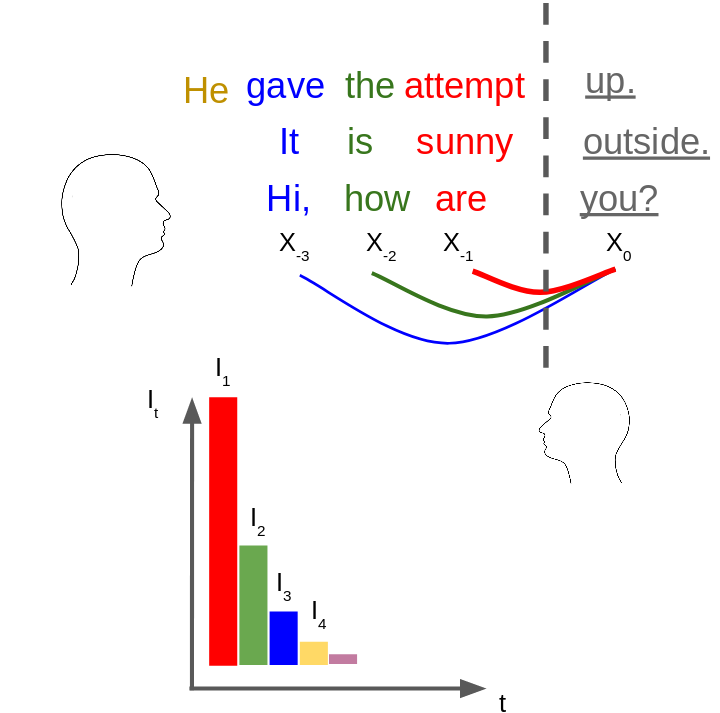
\includegraphics[width=0.4\textwidth]{figures-gdrive/mi-distance.png}
	(b)
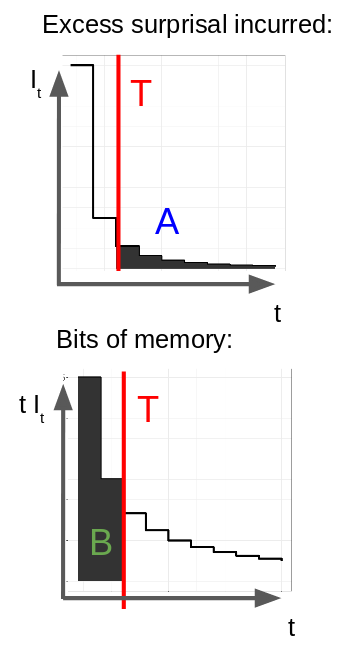
\includegraphics[width=0.2\textwidth]{figures-gdrive/theorem.png}
	(c)
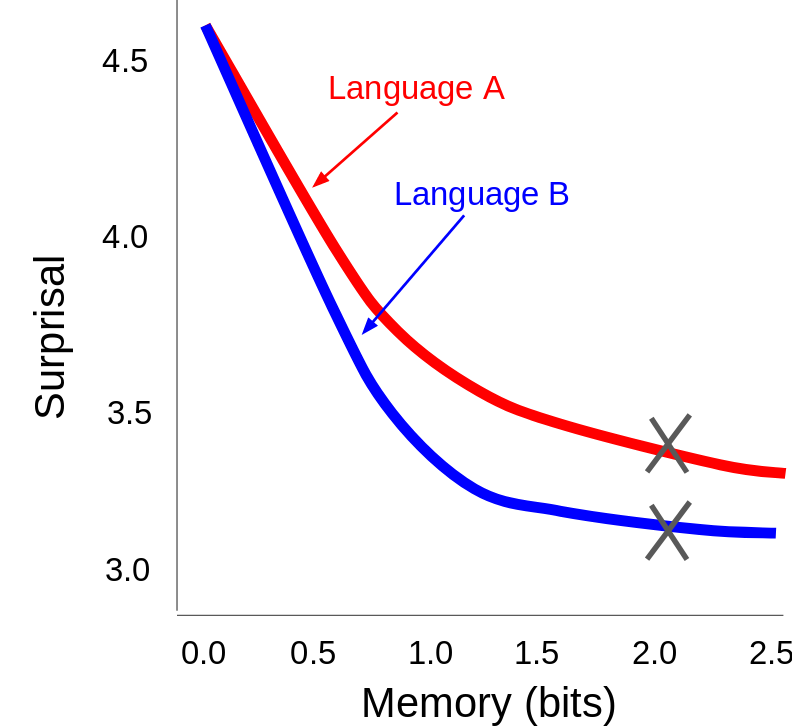
\includegraphics[width=0.2\textwidth]{figures-gdrive/tradeoff.png}
	\caption{
		(a) Conditional mutual information $I_t$ captures how much predictive information about the next word is provided, on average, by the word $t$ steps in the past.
		(b) Here we illustrate our theoretical result. We plot $I_t$ (top) and $tI_t$ (bottom) as functions of $t$. A listener using $B$ bits memory (bottom) to represent prior observations will incur at least $A$ bits of extra surprisal beyond the entropy rate (top). \note{there is t and T. COnfusing}
		(c) \jd{FILL OUT} \note{make the colors in (c) difefrenfr from this in (b). Do want to make clear what the mapping from (b) to (c) is. Maybe can even have a pair of the two (b) curves, and then show what they map on.}
}\label{fig:theorem}
\end{figure}


%TODO
%Let $I_t$ be the Conditional Mutual Information of two words $w_0, w_t$ conditioned on the intervening words:
%\note{hard to swallow for general audience. maybe can just use more straightforward less mathy language.}
%
%
%\note{Alternative:}
%A listener will experience average surprisal at least
%\begin{equation}
%	H[w_t| w_{<t}] + \sum_{t=T+1}^\infty I_t
%\end{equation}
%where $T$ is chosen to be the smallest $T$ for which $\sum_{t=1}^T t I_t \geq B$.
%\note{End alternative.}


%We prove that, for any integer $T > 0$, a listener encoding $\sum_{t=1}^T t I_t$ bits of memory will incur average surprisal at least $H[w_t| w_{<t}] + \sum_{t=T+1}^\infty I_t$.
%maybe multiple sentences in def of It?
%define math, AND give people intuition.












We now introduce our main theoretical result on memory-surprisal tradeoffs.





\begin{figure}
	\begin{center}
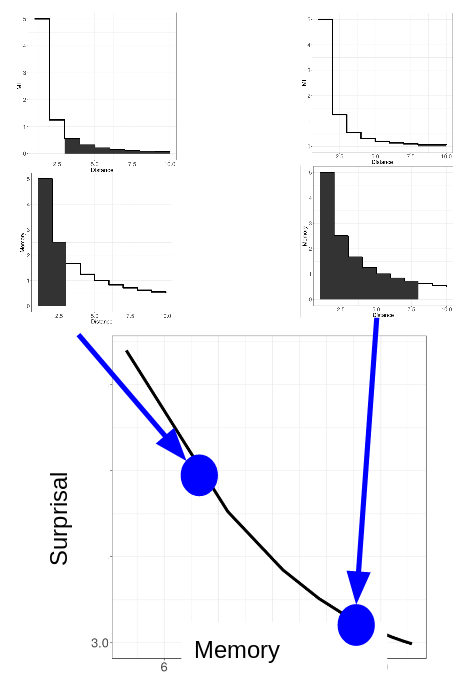
\includegraphics[width=0.45\textwidth]{figures/interpolate-curve.png}
\end{center}
	\caption{Estimating memory-surprisal tradeoff using the Theorem: We trace out the memory and surprisal values for all $T=1, 2, ...$, and linearly interpolate the curve.}\label{fig:interpolate}
\end{figure}







The proposition gives us a lower bound on the listener's memory-surprisal curve: Taking all pairs of memory $\sum_{t=1}^T t I_t$ and surprisal $H[w_t|w_{<t}] + \sum_{t > T} I_t$.
Then interplate linearly (justify this in appendix).
We obtain a curve in memry-surprisal plane, which is a lower bound on the memory demands of any listener at a given surprisal level.
We visualize this for the two processes from Figure~\ref{fig:basic} in Figure~\ref{fig:listener-tradeoff}.


\begin{figure*}
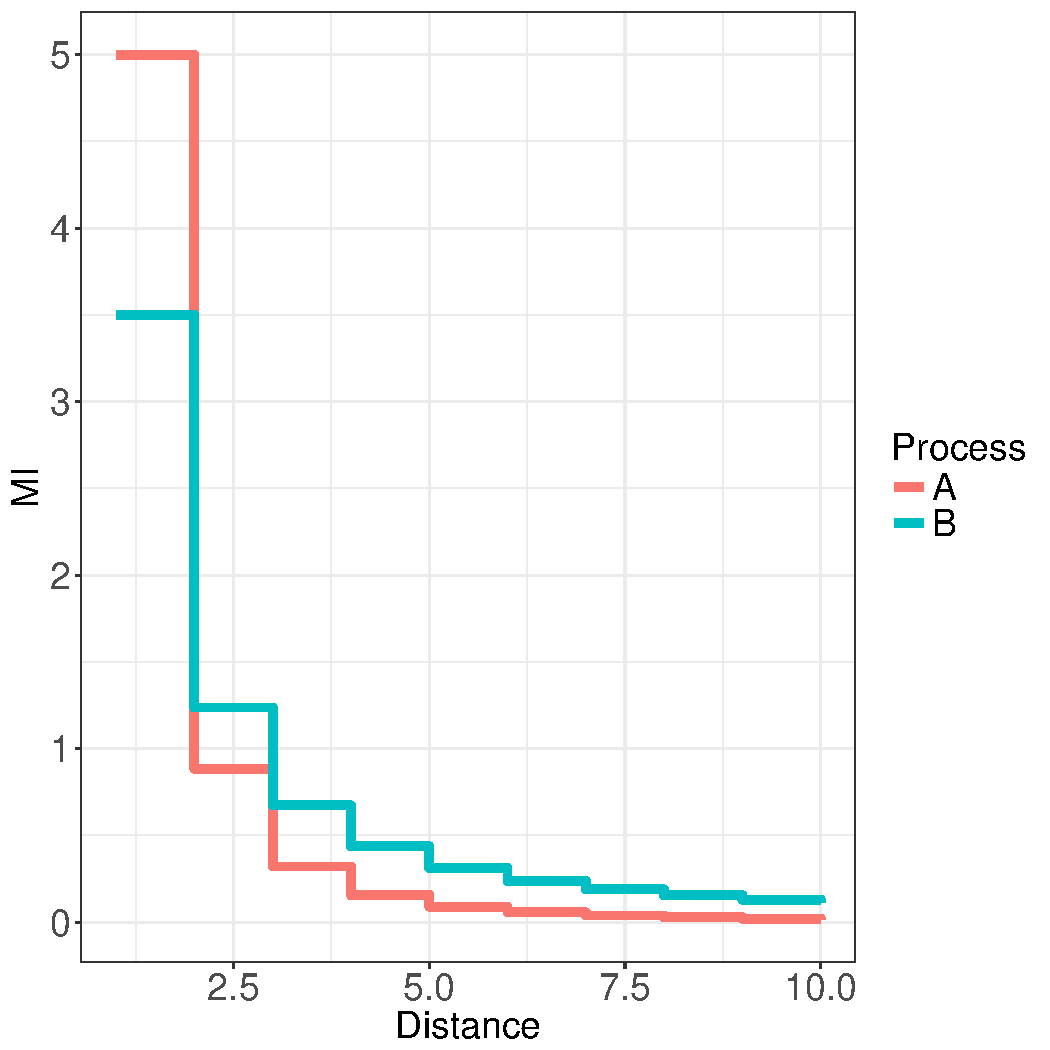
\includegraphics[width=0.45\textwidth]{figures/decay.pdf}
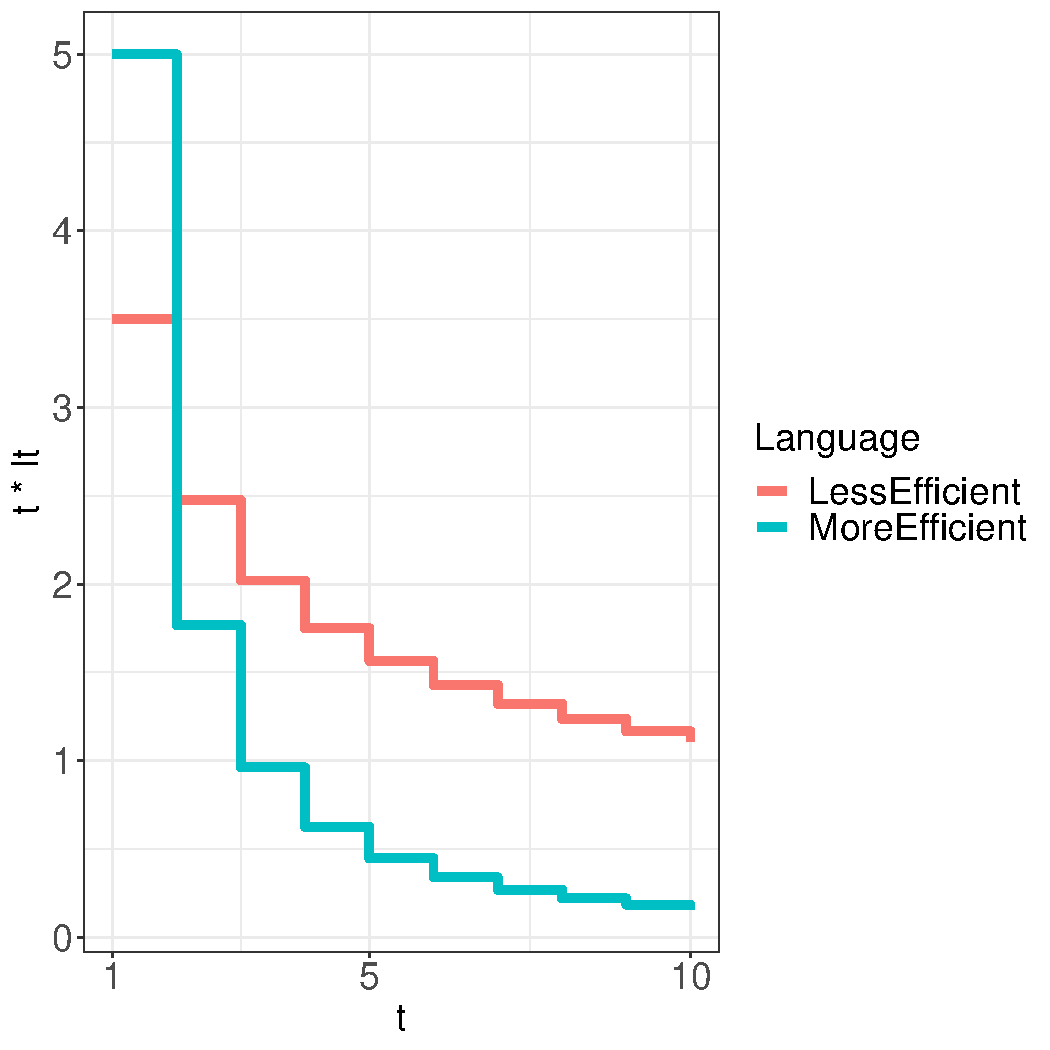
\includegraphics[width=0.45\textwidth]{figures/memory.pdf}
%
	\caption{Left: $I_t$ as a function of $t$, for two different processes. $I_t$ decays faster for the red process: Predictive information about the present observation is concentrated more strongly in the recent past. Left: $t \cdot I_t$ as a function of $t$ for the same processes. }\label{fig:basic}
\end{figure*}



\begin{figure}
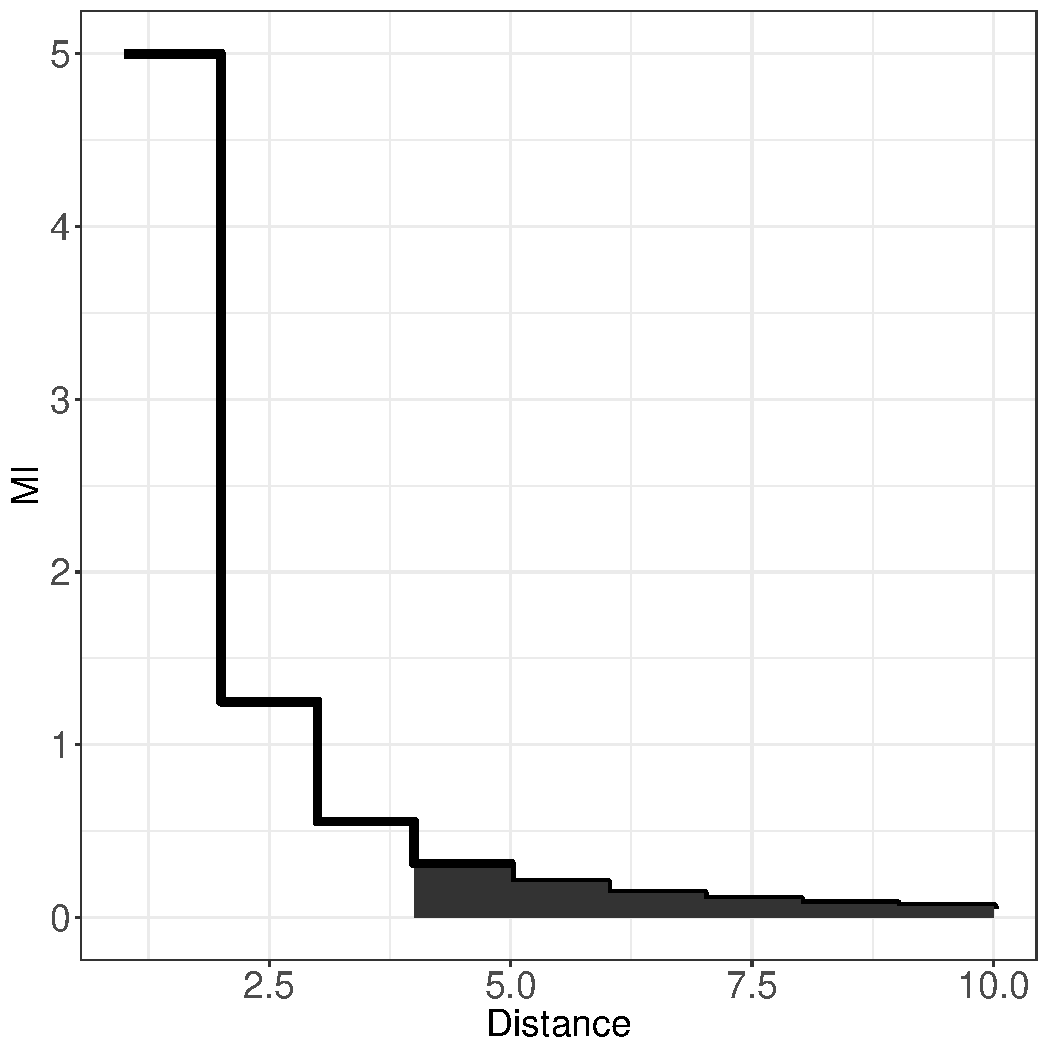
\includegraphics[width=0.45\textwidth]{figures/add-surp.pdf}
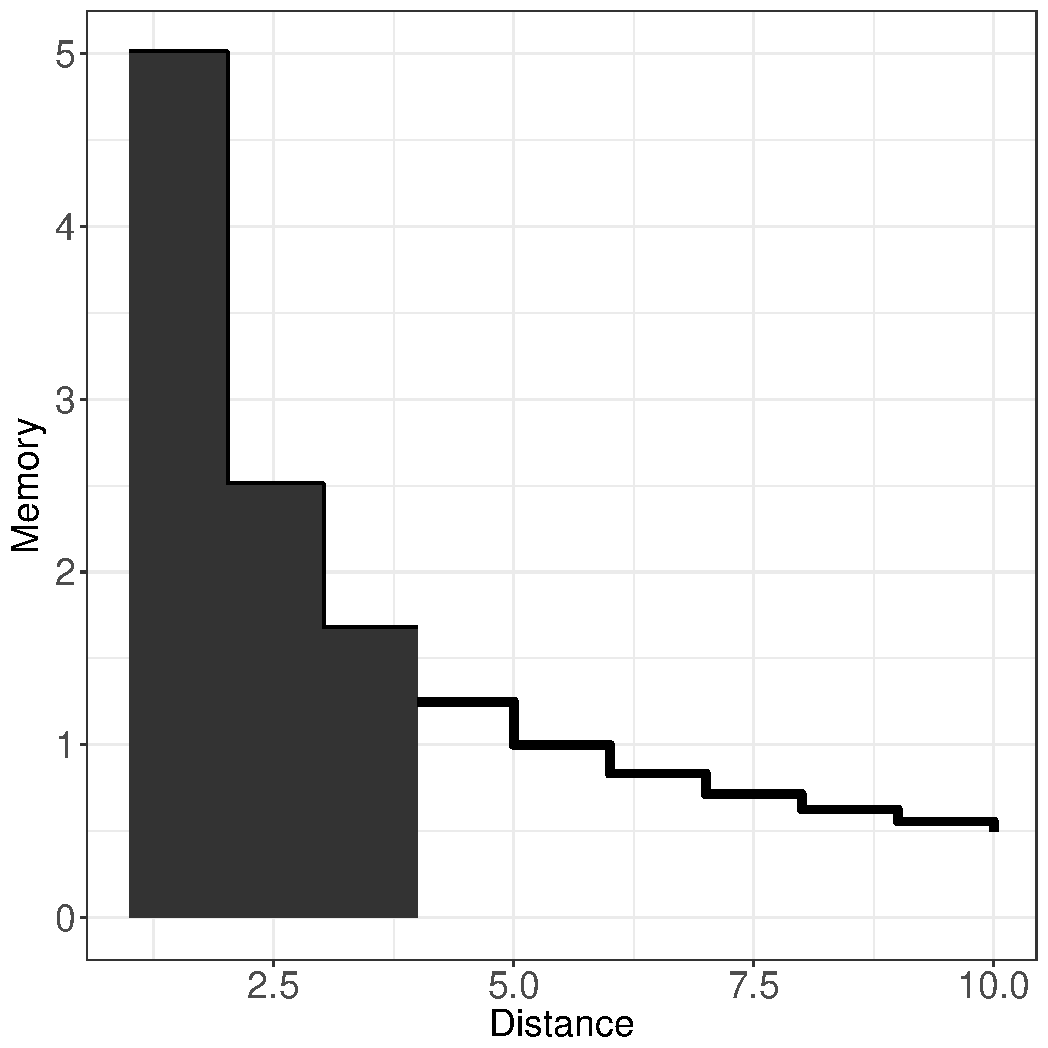
\includegraphics[width=0.45\textwidth]{figures/lower-mem.pdf}
	\caption{Illustration for Proposition~\ref{prop:suboptimal}. Listeners can trade off memory and surprisal: A listener only investing memory of the amount given by the black area on the right will incur at least the black area on the left in additional surprisal. In the given example, $T=4$. By varying $T$, the two areas describe the listener's memory-surprisal tradeoff curve.}\label{fig:listener-tradeoff-decay}
\end{figure}




\begin{figure}
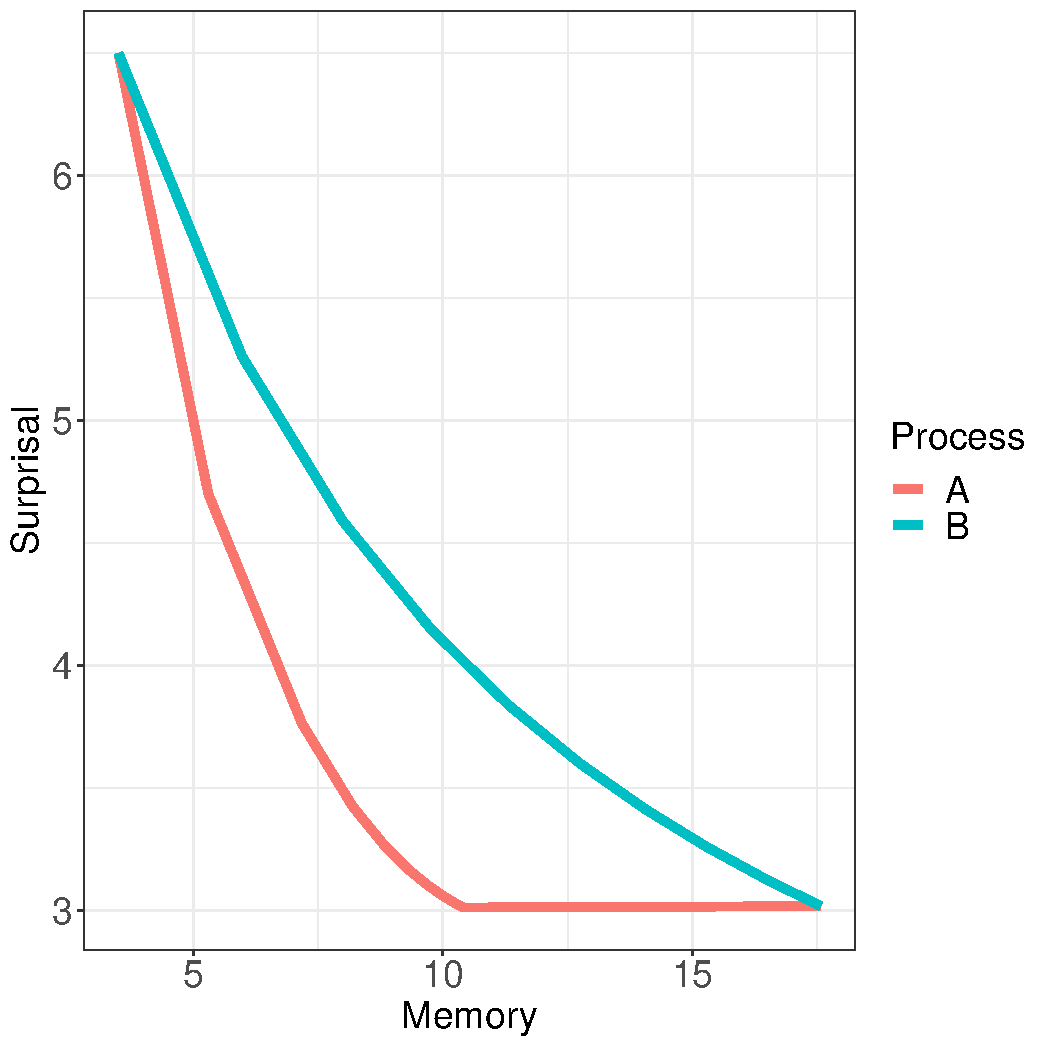
\includegraphics[width=0.45\textwidth]{figures/listener-tradeoff.pdf}
	\caption{Listener's memory-surprisal tradeoff for the two processes in Figure~\ref{fig:basic}. Recall that the red process had a faster decay of conditional mutual information. Correspondingly, this figure shows that a listener can achieve lower surprisal at the same level of memory load.}\label{fig:listener-tradeoff}
\end{figure}




%\subsection{Formal Analysis and Proofs}






\subsection{Information Locality}\label{sec:info-locality}

Due to the factor $t$ inside each term of the sum, carrying the same amount of information over longer distances requires more memory -- that is, modeling long statistical dependencies is more costly in terms of memory than modeling shorter ones.
This formalizes a general, assumption-free, link between memory and locality in language production.
In Section~\ref{sec:listener}, we will extend this analysis to listeners performing incremental prediction.
%incremental prediction.

%We will write $I_t$ as an abbreviation for $\operatorname{I}[w_t, w_0 | w_1, ..., w_{t-1}]$.
The proposition implies that memory is decreased if $I_t$ decreases quickly as $t \rightarrow \infty$ -- that is, if the contributions of long-term dependencies in the process are small.
In particular, memory load can only be finite if $I_t$ decreases fast enough for the infinite sum to converge to a finite value.
%This confirms the intuition that finiteness of memory entails that the contribution of long-term 

%\paragraph{Discussion}
%We have treated the process $(w_t)_t$ as a discrete-time process whose time steps correspond to words, but this is immaterial to the analysis.
%The analysis is not even restricted to discrete timesteps: We can replace thes sum in Proposition~\ref{prop:suboptimal} with an integral to get a continuous-time version.

We illustrate Proposition~\ref{prop:lower-bound} in Figure~\ref{fig:basic}.
We consider two processes A and B, where $I_t := 5t^{-1.5}$ for $A$ and $I_t := 3.5 t^{-2.5}$ for $B$.
The curves of $I_t$, as a function of the distance $t$, are shown in Figure~\ref{fig:basic} (left).
In both cases, $I_t$ converges to zero as $t$ grows to infinity. 
However, $I_t$ decays more quickly for Process A (red).
This means that predictive information about an observation is concentrated more strongly in the recent past.
In Figure~\ref{fig:basic} (right), we show $t\cdot I_t$ as a function of $t$.
Note that the area under the curve is equal to (\ref{eq:memory-bound}).
This area is smaller for the red process, as $I_t$ decays more quickly there.  





